\chapter{Introduction}

% Maybe start off as far back as "protein folding" ?
% What would I write though?
% Check out Misbehaving proteins the book.

% Broad theme: Protein folding, self-assembly, and its modulation ???
% Importance of protein folding -- structure - function paradigm
% Functions by binding with other proteins or ligands in the body.
% Ok, we also know about intrinsically disordered proteins that have well-defined functions in the human body.
% 
% But what about amyloid ... this common state that all proteins reach which results from protein aggregation

% The general problem of protein - structure and function
Perhaps one of the most remarkable phenomenon of nature is the ability of proteins to fold and self-assemble from a polypeptide chain into structures which impart their functions as molecular machines of life.

% Since the historical experiment performed by Anfinsen and colleagues which demonstrated that the structure of a folded protein is dependent on upon in its amino acid sequence and solvent environment, the protein folding problem has emerged as an important problem in biochemistry and biophysics.

% Protein interactions, and how protein function may be modulated by these interactions -- particularly solvent interactions.
Aenean orci erat, aliquet eu feugiat vitae, laoreet in justo. Aenean non dapibus leo. Pellentesque in nulla nec justo commodo varius ut congue ante. Aenean neque nibh, ornare sit amet tincidunt in, ullamcorper vitae risus. Aliquam rutrum porta suscipit. Aliquam erat volutpat. Aenean odio diam, vehicula sed interdum non, fringilla eu eros. Nunc ac diam arcu.


For many years, structural biologists focused their studies on proteins with well-defined folded states, and proteins capable of functioning without a unique folded state were largely sidelined.

% Protein misfolding and aggregation
However, in recent years, much attention have been focused on understanding what happens when proteins misfold, that is fail to achieve its proper folded structure necessary to carry out their normal physiological function.  Furthermore, the important of intrinsically disordered proteins, a class of proteins which do not adopt rigid 3-dimensional structures under physiological conditions, have gained much attention due to their roles in regulation, signaling.   Among these IDPs are a subset of proteins which are involved in numerous human diseases.  These proteins have been found to aggregate to form amyloid fibrils under certain solution conditions. Amyloid fibrils are widely known to be involved in many incurable diseases such as prion-related diseases, neurodegenerative diseases, Type II diabetes, and systemic amyloidosis. 


% It is also thought that amyloid fibrillar state may be the globally stable folded state for all proteins.

% Perhaps show a table here of all the proteins and diseases that they may be involved in.
% Columns Protein, has a structure?, disordered?, disease it is involved in.

\section{The amyloid state of proteins}
% A paragraph as a general introduction to amyloid.
% What's the general interest behind amyloid science -- why is amyloid important
% Here lead into a more detailed discussion about AD
% Role of amyloid in the human body

About 150 years ago, amyloids were defined as tissue deposits of extracellular filaments.\cite{Haass:2007db,Sipe:2000fs} These fibrillar deposits were microscopically visible, and sometimes even visible by eye in various organs in many seemingly unrelated human diseases.

Amyloid deposits all show specific optical behaviour (such as birefringence) on binding certain dye molecules such as Congo red.

% amyloid may be general to all proteins
The ability of polypeptide chains to form amyloid structures is not restricted to the relatively small number of proteins associated with recognized clinical disorders. Amyloid fibrils were observed to be formed in vitro by many other peptides and proteins, including well-known molecules such as myoglobin, and also by homopolymers such as polythreonine or polylysine.  
% This suggests that the amyloid state may be the globally stable for all polypeptides.

Although the ability of proteins to form amyloid fibrils appear to be generic, the propensity for a given peptide is highly dependent on the formation condition, and vary for different sequences. 

% The relative aggregation rates for a wide range of peptides and proteins correlates with the physicochemical features of the molecules such as charge, secondary-structure propensities and hydrophobicity. 

In a globular protein the polypeptide main chain and the hydrophobic side chains are largely buried within the folded structure. Only when they are exposed, for example when the protein is partly unfolded (for example, at low pH) or fragmented (for example, by proteolysis), will conversion into amyloid fibrils be possible. 


% How is amyloid formed
% kinetics of aggregation ?
Amyloid fibrils are formed via a complex aggregation pathway. Initially, monomers aggregate to form oligomers with different morphologies which exists in equilibrium with amyloid fibrils. Some of these oligomers are on-pathway to fibril formation, while others themselves may be end-points of the aggregation pathway. Biochemically, fibrils are protease resistant and are insoluble in the presence of Sodium dodecyl sulfate (SDS).


Amyloid fibrils have been observed to form via a two-step nucleation-polymerization process, a behaviour that is typical of nucleated processes such as crystallization.  In the nucleation phase, a lag phase occurs where energetic barriers of aggregation must be overcome to form the initial aggregation nucleus. Seeding, a process where preformed aggregates is introduced into solutions, may eliminate the lag phase.  Following the lag phase, free monomers may bind to the nucleated aggregates and polymerize into mature fibrils.\cite{Murphy:2002fe} 


\subsection{Fibrils}

\begin{figure}
  \centering
  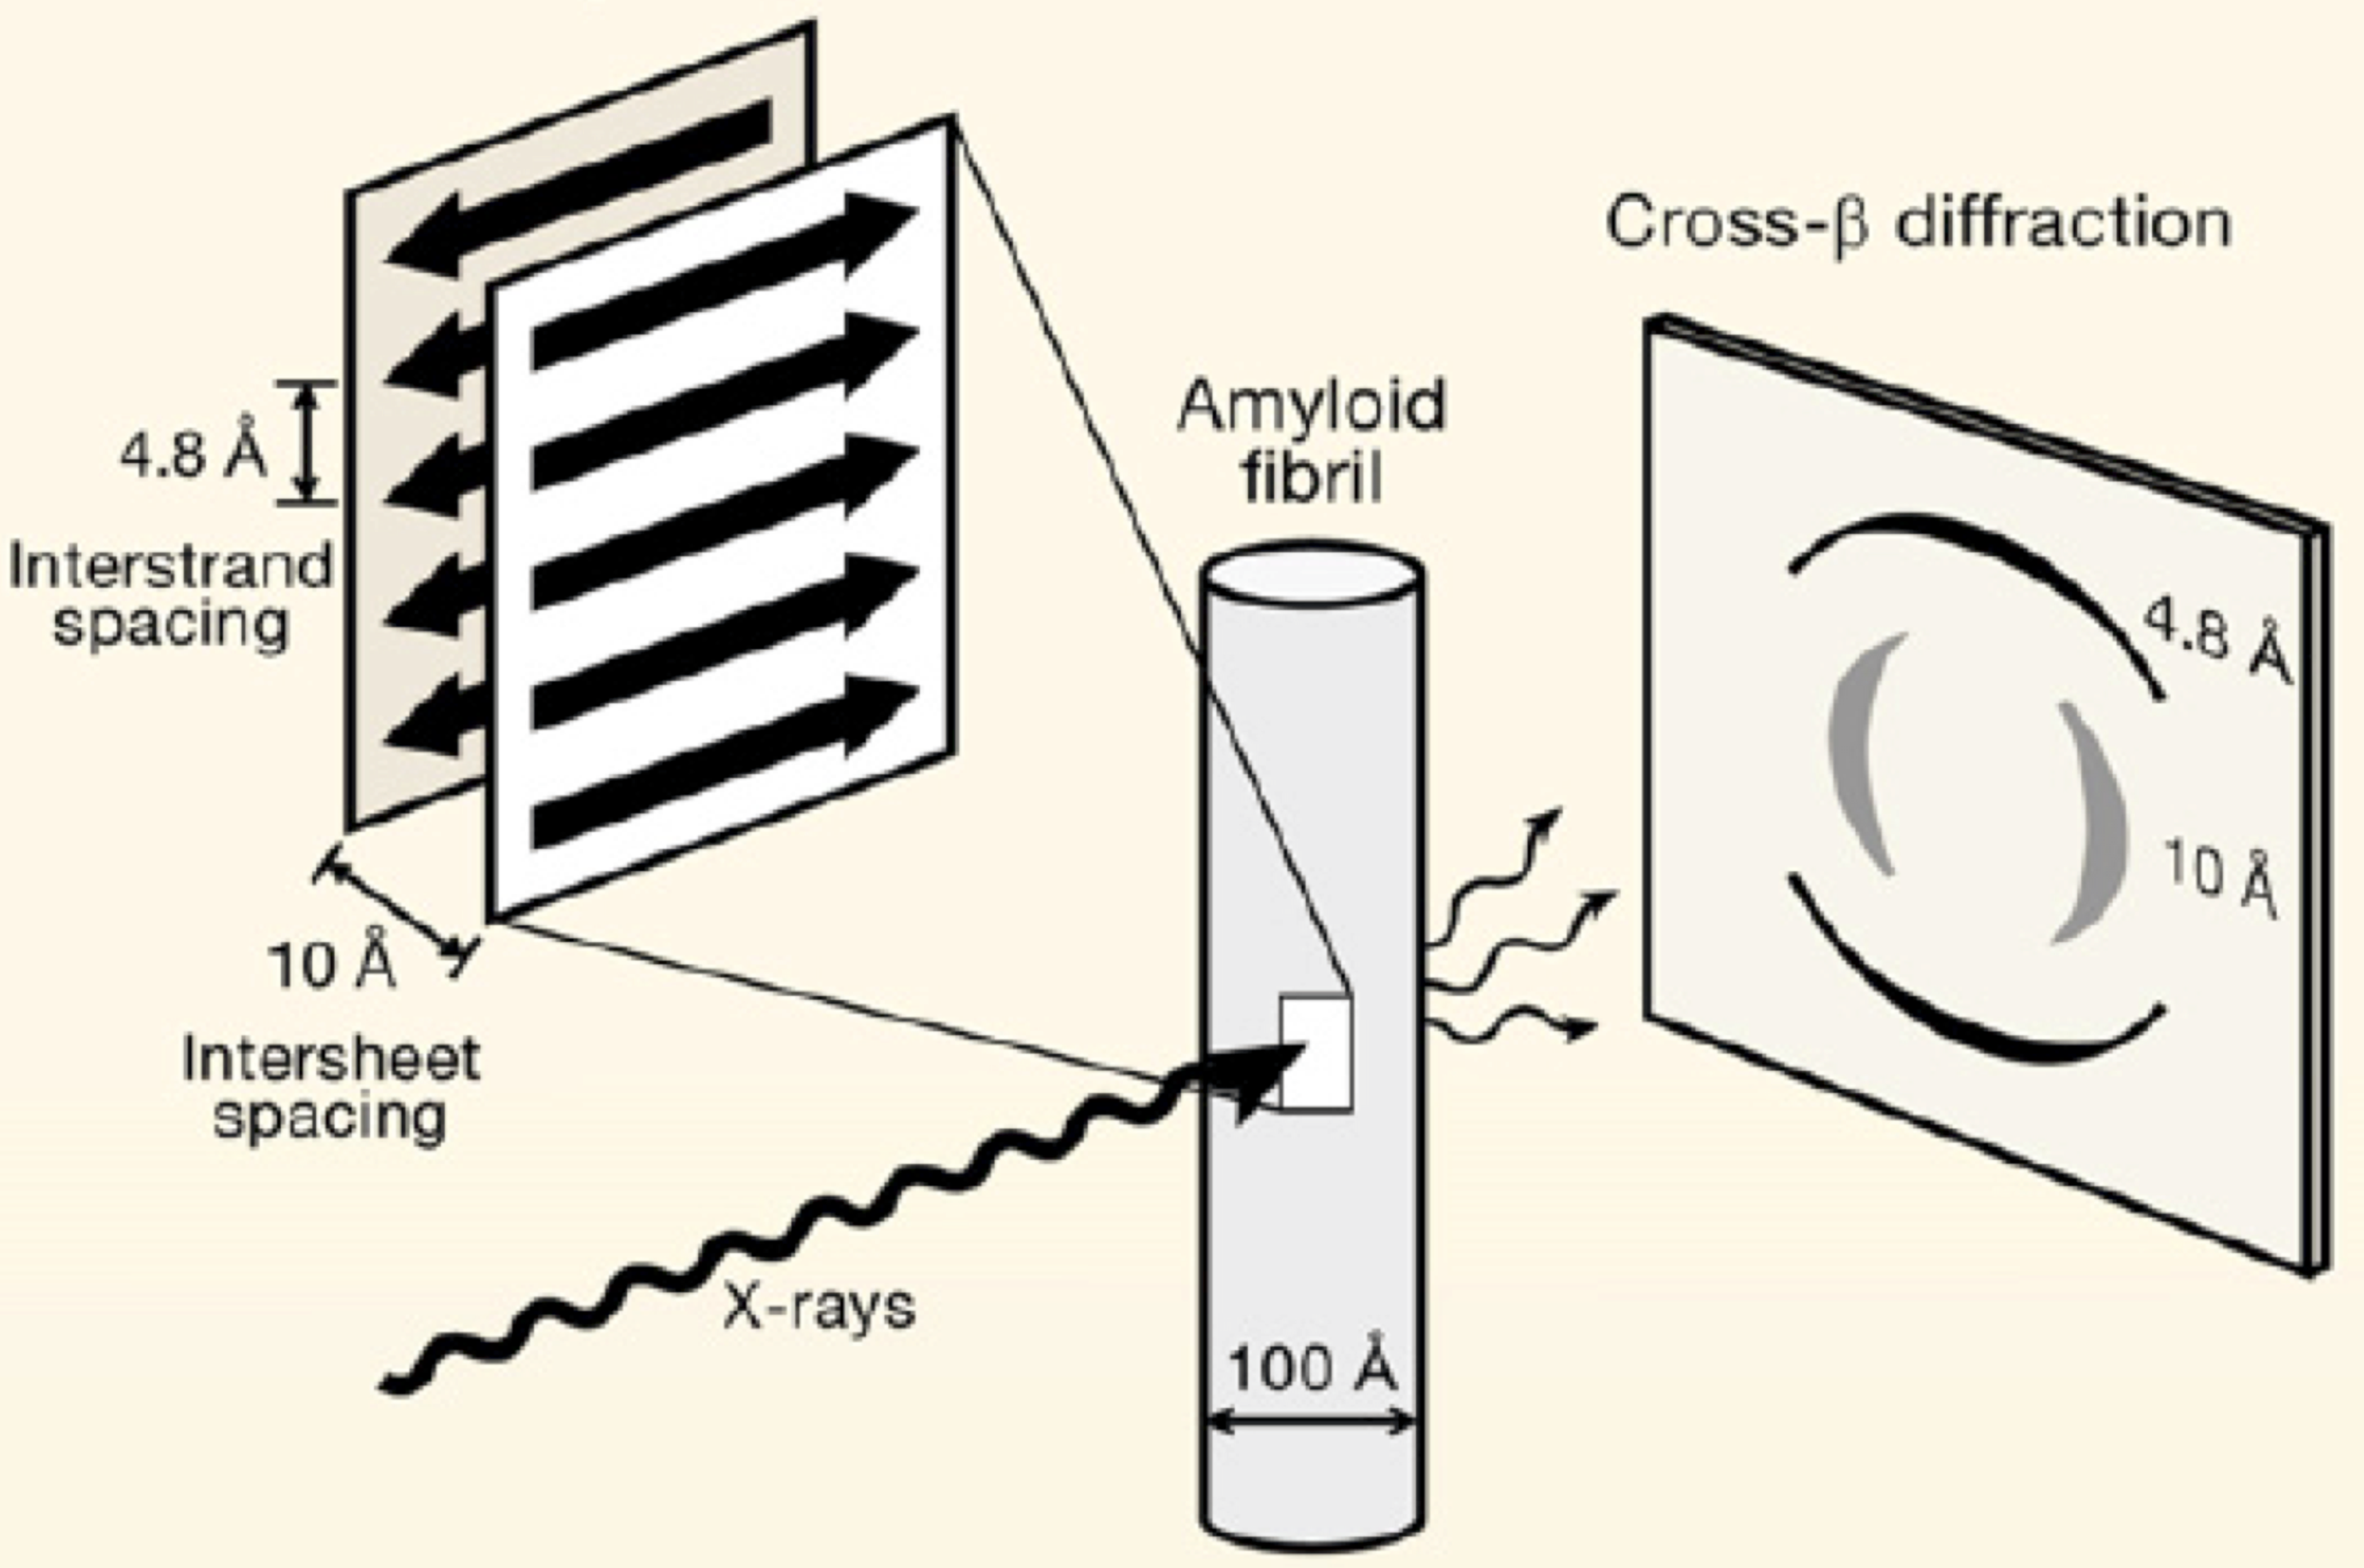
\includegraphics[width=6in]{figures/introduction/fibril_structure_diffraction.pdf}
  \caption[Characteristic cross-$\beta$ spacings from X-ray fibre diffraction studies of amyloid fibrils]{This is adapted from Eisenberg, 2012}
  \label{fig:fibril_diffraction}
\end{figure}

% Finding a treatment for AD and other fatal neurodegenerative diseases motivated many biochemical and biophysical studies of the amyloid state. 

Despite having dramatically different sequences, amyloid fibrils formed from different polypeptide all adopt a similar structure called the \crossbs.  The first structural studies of fibrils using X-ray fiber diffraction showed that a \crossb\ is characterized by a 4.8\angstrom\ interpeptide, and 10\angstrom\ intersheet spacing. XXX add more details to this description. XXX [Need to have a figure which shows this diffraction pattern, and EM data with cartoon model.] This defining characteristic of \crossb\ have now been adopted by biophysicists as an indication for the presence of amyloid fibrils.


Under the transmission electron microscope (TEM), fibrillar structures typical of many aggregates are visible as long, unbranched, often twisted ribbon-like structures nanometers in diameter (Figure~\ref{fig:fibril_TEM_SSNMR}). Independent measurements of fibrillar structure using different instruments have all confirmed the presence of \crossbs as the core structure of amyloid fibrils. (Figure~\ref{fig:fibril_diffraction})

% Other measurements 
% MPL Mass per unit length

Although \crossb\ is widely known, due to the insolubility and inherent non-crystalline nature of amyloid fibrils, the details of the fibril structure at the molecular level remained elusive until recently. Advances in solid-state NMR (SSNMR) and X-ray crystallography in the last decade have made major contributions to our knowledge of the molecular structure of amyloid fibrils.

\begin{figure}
  \centering
  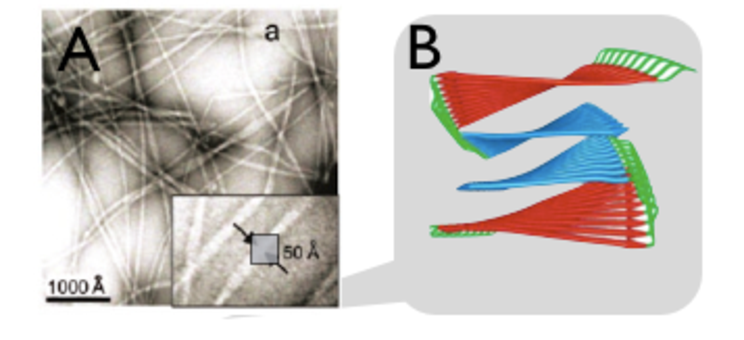
\includegraphics[width=6in]{figures/introduction/fibril_TEM_SSNMR.pdf}
  \caption[Characteristic cross-$\beta$ spacings from X-ray fibre diffraction studies of amyloid fibrils]{A Example EM images of oligomers.  Adapted from Bitan G. et al. 2003 and Walsh D. 1999 C TEM image of fibrils D SSNMR model proposed by Tycko et al.}
  \label{fig:fibril_TEM_SSNMR}
\end{figure}

% Describe the molecular structure of \abeta\ amyloid fibrils. 
% Briefly mention the techniques that can be used to obtain structural information of amyloid fibrils. 

% SSNMR
The initial molecular model of an amyloid fibril was for \abeta40, the peptide involved in Alzheimer's disease.  A SSNMR study on the amyloid fibrils of A$\beta$40 was done by Tycko et al in 2002. XXX The fibril core of \abeta40 involves the stretch sequence XXX-YYY. It is thought that residues A to B is disordered. The core fibril unit consists of a parallel in-register \bsheet, where each strand is a \bhairpin\ with peptide-peptide backbone hydrogen-bond along the long axis of the fibril. Figure~\ref{fig:fibril_TEM_SSNMR}


% X-ray structures
Furthermore, small peptide fragments that have characteristics of amyloid fibrils, which are also amenable to single crystal X-ray diffraction analysis have demonstrated similar type structures from those studied using SSNMR.  These structures obtained by X-ray crystallography have been described to have a dry interface with stacked sheets. (Figure~\ref{fig:fibril_xray_model})

\begin{figure}
  \centering
  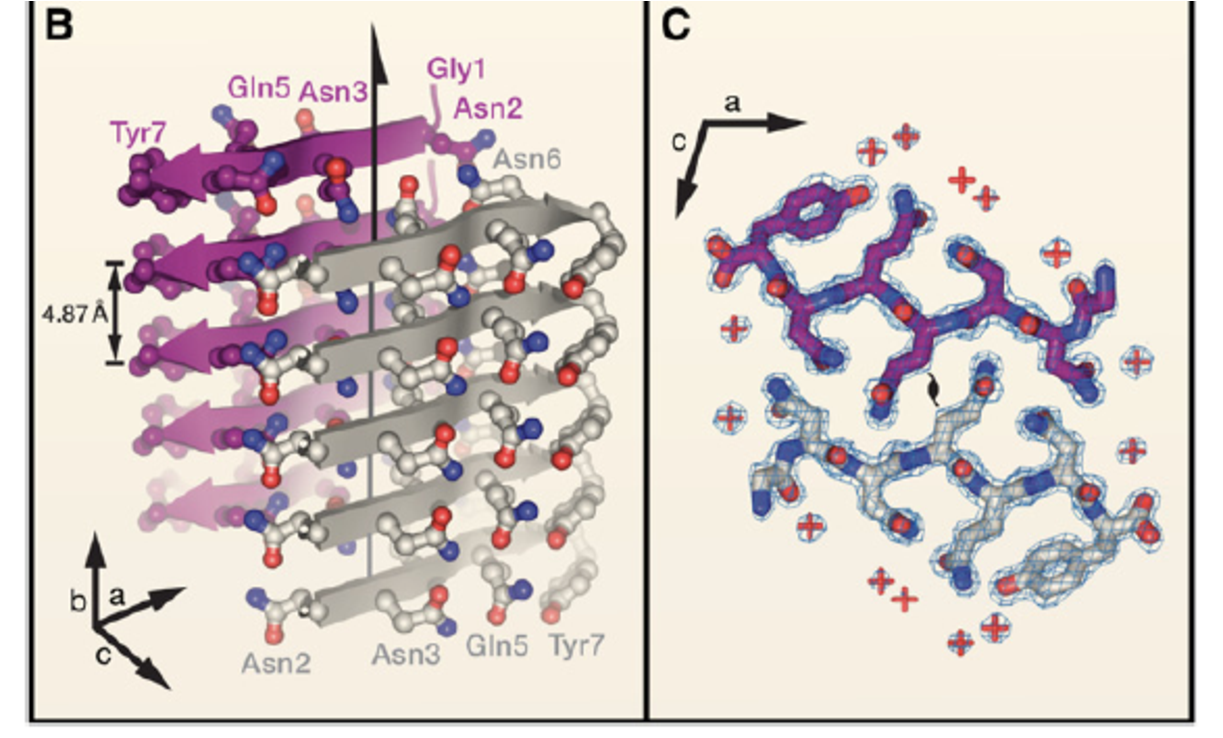
\includegraphics[width=6in]{figures/introduction/fibril_xray_model.pdf}
  \caption[Characteristic cross-$\beta$ spacings from X-ray fibre diffraction studies of amyloid fibrils]{This is adapted from Eisenberg, 2012}
  \label{fig:fibril_xray_model}
\end{figure}

% What do all fibrils have in common?
% Organization of the peptide backbone into beta-sheets; sheet stacking
The ubiquitous presence of a \crossbs supports that the organization of the peptidic backbone, common to all proteins, in to \bsheets\ is a major determinant of the fibrillar structure. Moreover, the proposed structures (some described above), indicate that the core region is composed of two to four sheets that interact closely with each other.

% I don't think I will talk about the twisting of the sheets too much.
% An interesting feature of these sheets is that they appear to be much less twisted than ex- pected from the analysis of the short arrays of β-strands that form β-sheets in globular protein structures. This feature was first proposed from cryo-EM and has been supported by Fourier transform infrared (FTIR) analy- ses (48, 61).

\subsection{Polymorphism of fibrils}

% Even fibrils formed from a single peptide can exhibit polymorphism .
Although all fibrils share the \crossbs, individual fibrils exhibit polymorphism at the molecular level which is dependent upon the experimental conditions under which they are formed.  % (Figure~\ref{fig:fibril_diffraction})
Fibrils may vary in the length of the beta-strand involved, side chain orientation. 

\subsection{Non-fibrillar oligomers}
\begin{figure}
  \centering
  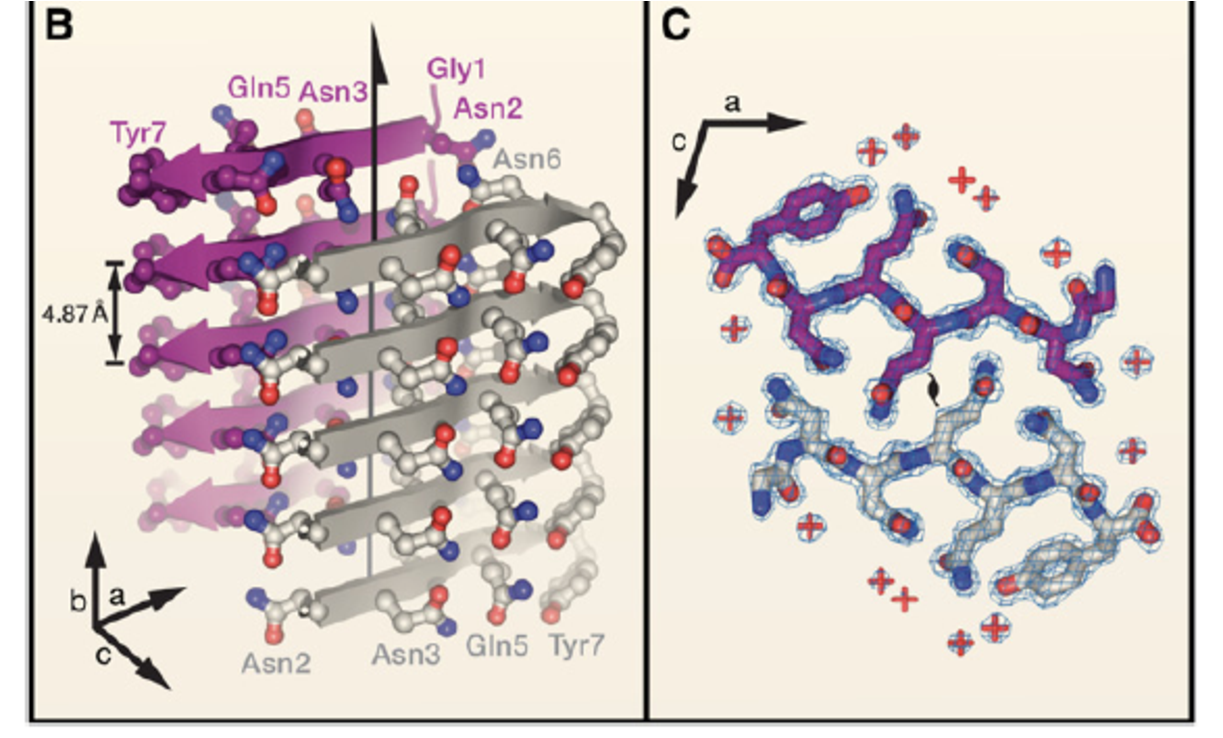
\includegraphics[width=6in]{figures/introduction/fibril_xray_model.pdf}
  \caption[Characteristic cross-$\beta$ spacings from X-ray fibre diffraction studies of amyloid fibrils]{This is adapted from Eisenberg, 2012}
  \label{fig:fibril_xray_model}
\end{figure}

Due to their structural disorder and their insolubility, molecular details of oligomers have been challenging to obtain using current structural determination techniques. 

EM and AFM experiments have shown that transient, unstable particles may appear prior to the formation of fibrils. In particular, soluble \abeta\ prefibrillar assemblies that are annular, spherical, or curvilinear in shape have been reported in literature.REF Protofibrils, in particular, are curvilinear, filamentous structures that are smaller than mature fibrils and are approximately 5-10 nm in diameter.9 Furthermore, protofibrils bind to dyes Thioflavin T (ThT) and Congo Red (CR), suggesting the presence of substantial β-sheet content.9, 13-15 Although some of these particles may be \bsheet-rich, they are morphologically distinct and are typically much smaller than fibrillar structures. Figure~\ref{fig:oligomers}

Despite the importance of these prefibrillar species in causing neurodegeneration, their molecular structures are still not known. However, a recent SSNMR study demonstrated that a late stage, neurotoxic Aβ40 spherical intermediate contained fibril-like β-sheet structure.16

[ Recent data show that non-fibrillar oligomers may contain fragments which are fibril-like in morphology. Most recently a study have shown that oligomers of \abeta\ ]
[ Should briefly read up on the book chapter by Pat Walsh]

\subsubsection{Amyloid Toxicity}
% I think outline some of the ideas / hypothesis about the link between amyloid and disease, but don't go into what people speculate or data on toxicity. It is related, but this is out of the scope of your thesis.

	% Key question in the field: What is the toxic species?
Multiple lines of research have identified oligomers as a likely causative agent for neuronal cell death. By contrast, the monomeric and fibril forms are thought to be less toxic than oligomers. It is hypothesized that soluble oligomers may cause toxicity by perturbing the integrity of cellular membranes through binding and disrupting the lipid bilayer (perhaps by making them ion permeable). \cite{Walsh:2007fu}

% Include a paragraph about amyloid formation and lipid membranes

% Understanding the toxicity or finding out whether there is a toxic species in part validates the amyloid hypothesis. 

% Here can lead into AD by saying well ... a widely known disease, where amyloid oligomers are thought to directly play a role in the disease process is AD.  

\section{Alzheimer's Disease}
One of the most well-known diseases involving amyloid formation is Alzheimer's Disease (AD), a devastating neurodegenerative disease that is most common cause of dementia in persons of age 65 or older.

% Pathological characterization
\begin{figure}
  \centering
  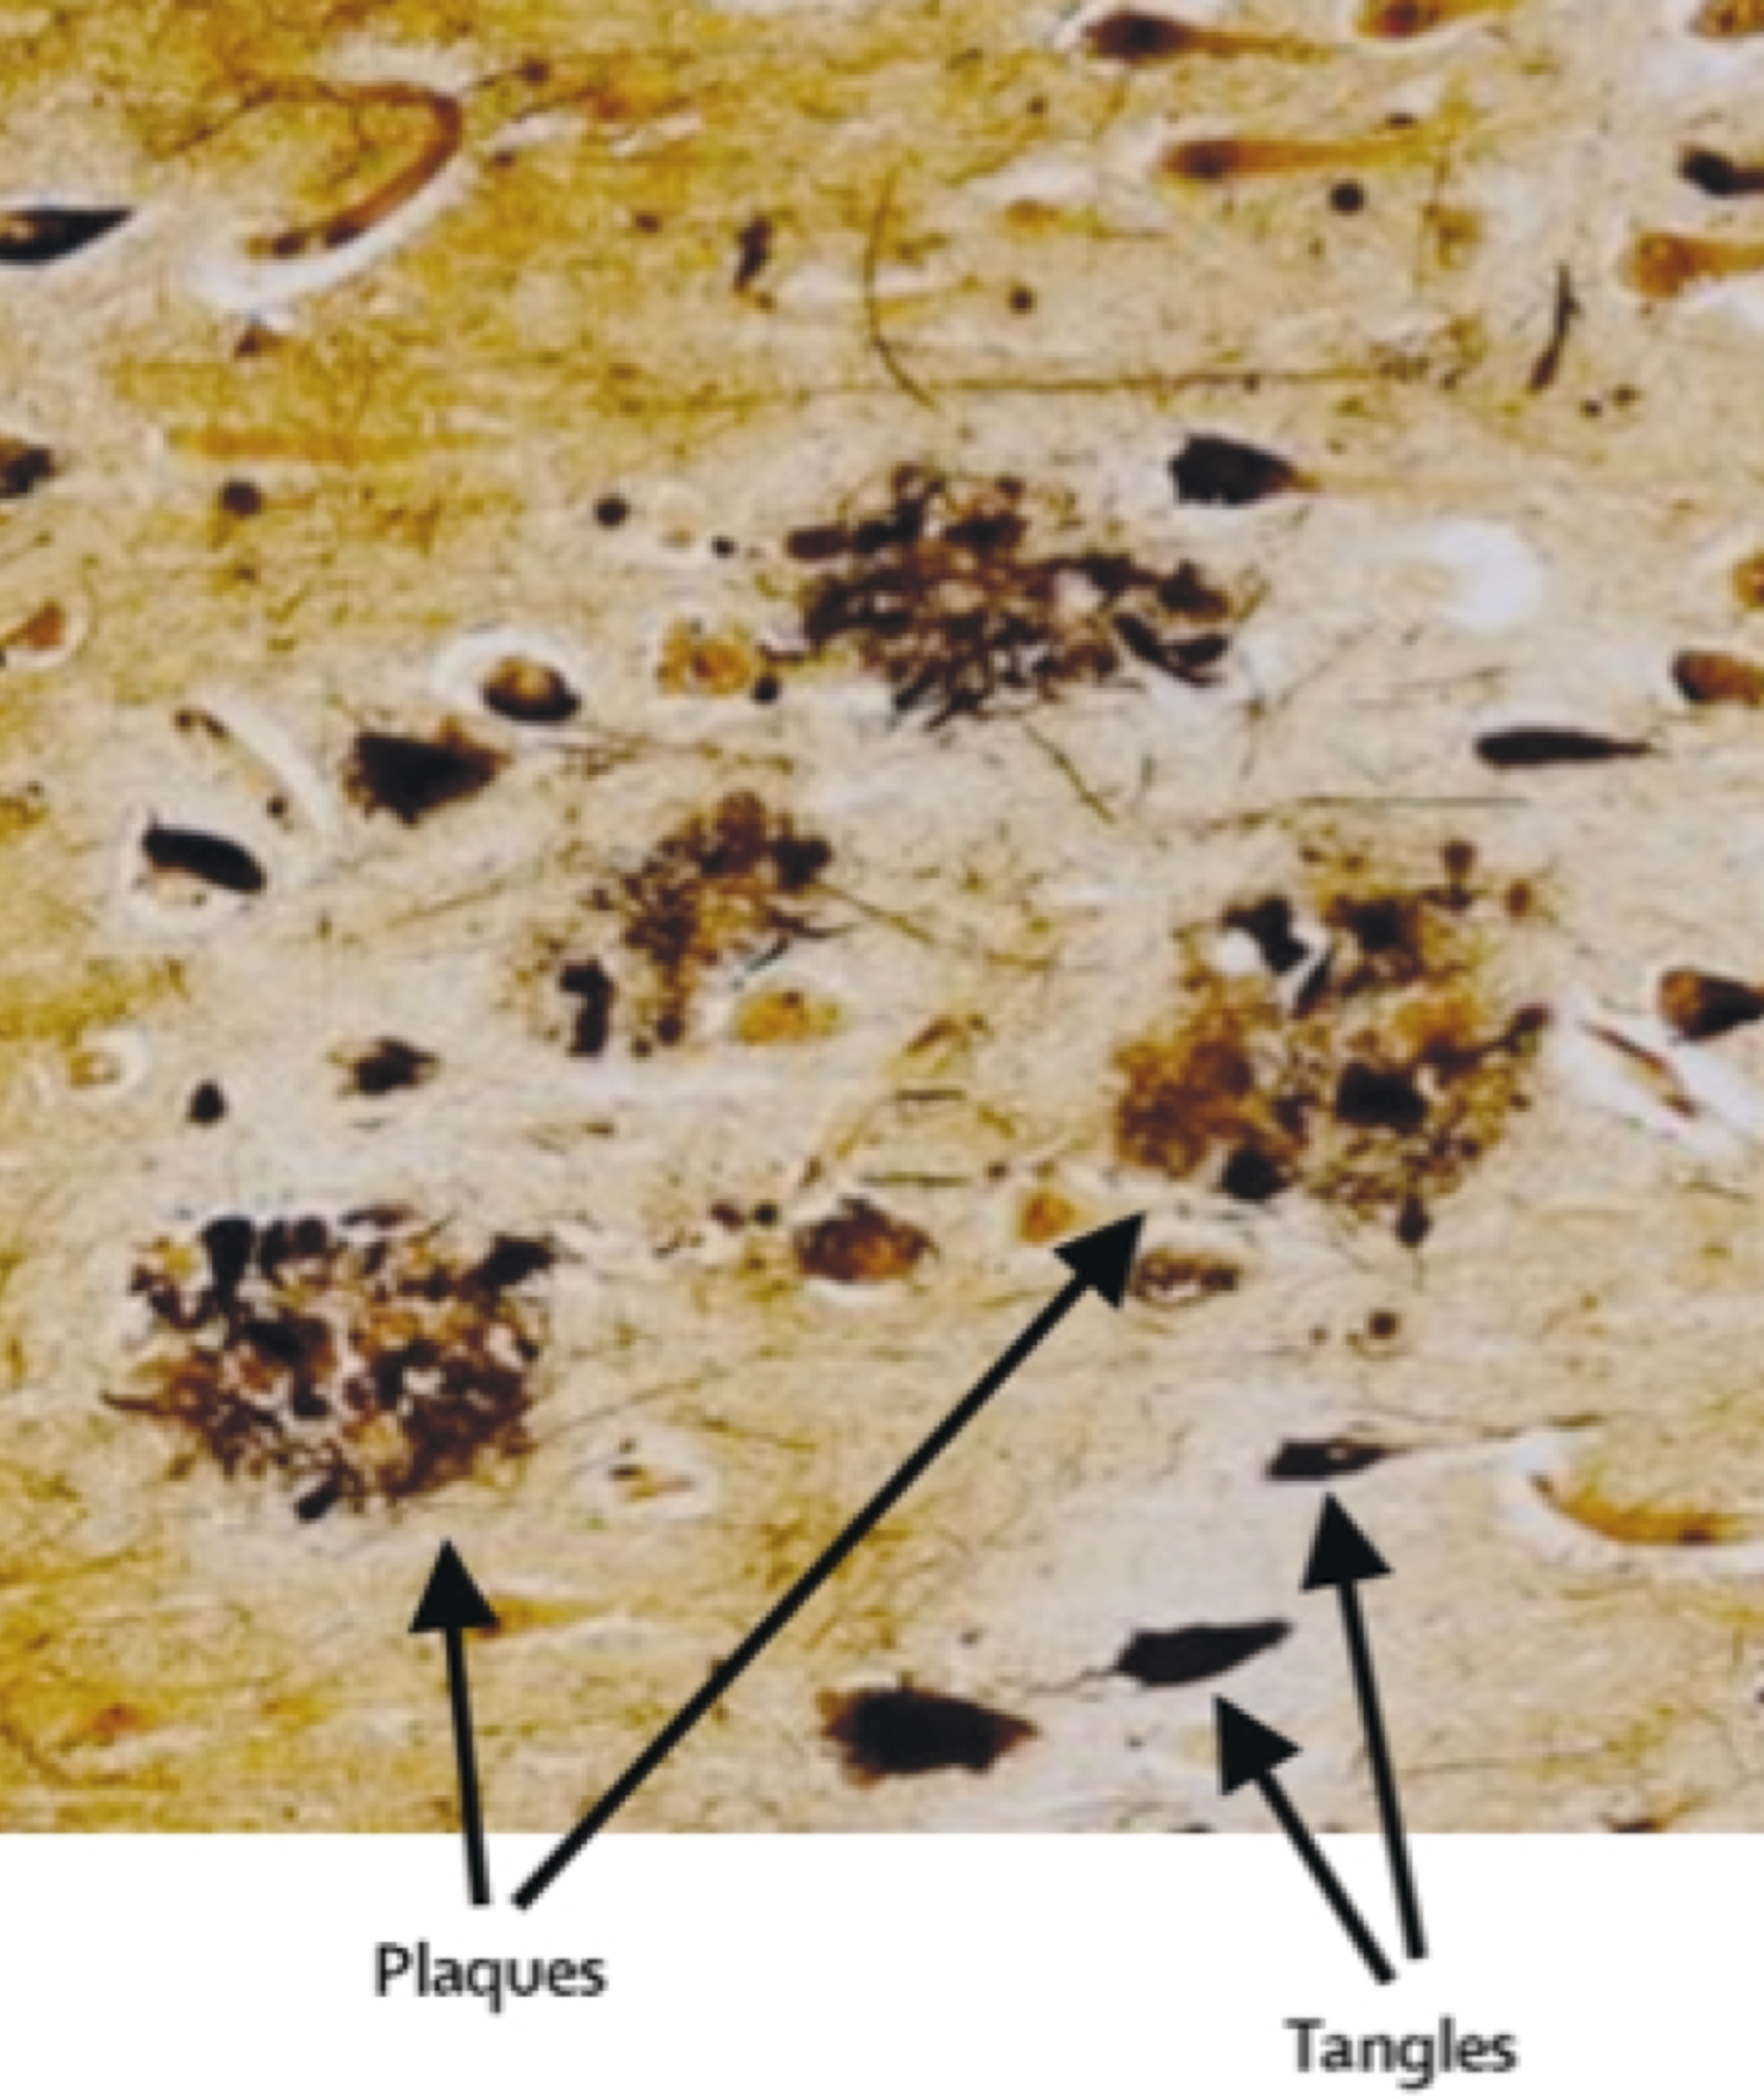
\includegraphics[width=6in]{figures/introduction/AD_tissue_pathology.pdf}
  \caption[Image of lesions formed by plaques and NFTs on brain tissue]{This is adapted from Blennow, 2006}
  \label{fig:AD_tissue_pathology}
\end{figure}

Upon examination, the brains of deceased AD patients show significant neuronal dystrophy.  Pathologically, AD is characterized by the presence of extracellular deposits of senile plaques and neurofibrillary tangles, which appear as lesions on stained neuronal tissue under light microscopy.(Figure~\ref{fig:AD_tissue_pathology})

Although it has been more than one hundred years since Dr. Alois Alzheimer first presented the association between the presence of neuronal plaques and the clinical symptoms of presenile dementia characteristic of Alzheimer's disease (AD), the exact relationship between the two is still under much contention.  It was not until in the 1980s, the protein \abeta\ was identified as the largest component of plaques. % How is Abeta produced ? Is it only involved in Abeta? What's the physiological role of Abeta?

The presence of amyloid plaque deposits in brains of deceased dementia patients led to the formulation of the long-standing amyloid hypothesis, which posits that amyloidogenesis of \abeta\ plays a key role in the initiation of AD. XXX

Although both plaques and NFTs appear together, many studies have indicated that NFTs plays a secondary role to \abeta\ in the pathogenesis of AD.
% More details on evidence which show that NFTs are not likely the causative species. Knock out mouse models ... mice do not develop AD, and instead develop tau pathologies  NFTs have also been shown to be affected by \abeta\ production.

% should I include more details on how Abeta is known to be produced in the body?
Monomeric \abeta\ is an approximately 4 kDa peptide produced by intramembrane proteolytic cleavage of the larger amyloid-$\beta$ precursor protein (APP) and is produced constitutively as part of the normal cellular metabolism.\{Selkoe, 2002 \#222\} APP is sequentially processed by the aspartyl proteases $\beta$-secretase and $\gamma$-secretase, where depending on the position of the cleavage by $\gamma$-secretase, a pool of \abeta peptides of lengths varying from 38 to 43 residues are produced. The peptides spanning residues 1-40 (\abetaforty) or 1-42 (\abetafortytwo) are predominantly found in AD-associated plaques. Neuritic plaques is composed of mainly \abetafortytwo, whereas \abetaforty\ is more commonly found in cerebralvascular plaques.

Multiple lines of evidence indicate that \abetafortytwo is likely to be the more deleterious form of \abeta. Genetic studies showed that mutations which cause early-onset AD also in turn increases the ratio of \abetafortytwo to \abetaforty.\cite{Hardy:1997tu} Moreover, in vitro, \abetafortytwo\ displays significantly higher propensity for aggregation than \abetaforty, despite differing by only two amino acids. In addition, \abetaforty\ and \abetafortytwo\ also have distinct aggregation pathways in vitro: \abetafortytwo is found to form a morphologically more diverse population of intermediate oligomers than \abetaforty.\cite{Bitan:2003ut}

% What about mice studies?

\abeta\ aggregates is present in a variety of morphologies in the brain. Although plaques are often visible in the dementia patients, the plaque load does not correlate with disease progression and severity, a puzzling aspect of AD.  Instead, synaptic loss correlated well with the concentration of soluble \abeta\ oligomers in the brain.

Currently there is a lack of treatment which targets the underlying disease. Most approved treatments today for AD only mitigates cognitive symptoms.  The vast number of structural and biochemical studies on amyloid structure have been crucial for the development of potential therapeutics for Alzheimer's disease.

%  Drug development for Alzheimer's has been on preventing amyloid aggregation and decreasing amyloid production. We will discuss this in more detail in later section XXX.
% Talk about how important it is to develop drugs for these amyloid disorders ... particularly for AD ... because it not only is a great economic burden on society, but a growing epidemic....

% \subsubsection{Other disorders}
% % Perhaps not enough to make it into its own subsection
% In addition to AD, other neurodegenerative diseases have been shown to involve the presence of amyloid.  Parkinson's disease, Huntington's, Prion disorders (Mad cow).  These diseases and their pathology are reviewed elsewhere and are beyond the scope of the thesis.
% I think I will not mention these things in detail in my introduction


\section{Amyloid Inhibition by small molecules: A promising method of treatment for AD}
% Cure, method of prevention; is there hope?

% In this section, I will provide an overview of some of the challenges to overcome when developing a small molecule therapeutic for Alzheimer's disease.  Furthermore, using this information, I will motivate why inositol is an exciting avenue to explore.

% Amyloid inhibition as a treatment for Alzheimer's disease and related amyloid disorders. 

% Briefly mention non-small molecule putative therapies which also acts via amyloid inhibition. The focus of this thesis will be on small-molecule amyloid inhibition.

% Use this as a transition into amyloid inhibition
% AD presents as a major economic and health burden to modern society.  With the longevity of our population, AD is approaching epidemic proportions with no cure or preventative therapy available.\cite{Blennow:2006wd}

Amyloids are attractive drug targets. Small molecules which targets amyloids may be an effective method of treatment for amyloid disorders because of the potential to treat the underlying disease. Through in vitro screening, many small molecules have been found to effect the amyloid aggregation pathway.  Some were demonstrated to inhibit amyloid fibrils, where as others were shown to arrest or reduce oligomer formation.
  
% Here I can take a cue from Justin Lemkul`'s recent review paper.
% Talk about the different kinds of small molecules that have been found to inhibition amyloid formation.  Here I will also provide a summary of what people know about the mechanism by which they inhibit amyloid formation.
Pharmacological perspective of the challenge of developing an Alzheimer's drug. In order to effectively treat Alzheimer's and other neurodegenerative diseases, small molecule drug candidates must pass the blood brain barrier at sufficient concentrations for inhibition.  This is difficult to achieve.
      
In vitro screening has led to the discovery of a large number of small-molecules which were found to affect the amyloid aggregation pathway. Many of these small molecules are thought to act by directly binding to amyloidogenic peptides and aggregates.

\begin{figure}
\centering
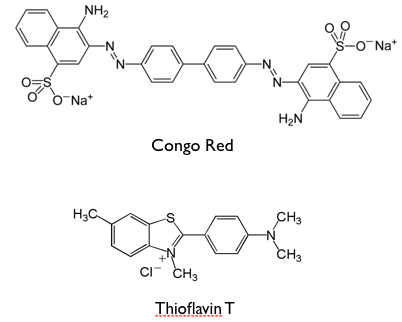
\includegraphics[width=3in]{figures/introduction/dyes.png}
\caption[Small molecule binders]{Amyloid binding dyes Congo Red and Thioflavin T}
\label{fig:amyloid_dyes}
\end{figure}

\subsection{Dye molecules}
Among the first molecules known to bind amyloid fibrils were dyes, Thioflavin T (ThT) and Congo Red (CR) used to identify their presence.

Early histological detection of amyloid binding was done using congo red, where upon binding fibrils exhibit red-green birefringence. Congo red requires the use of polarized light microscopy, a laborious process, and the interpretation of the birefringence is often not reproducible.

Thioflavin-T (ThT) is a benzathiole fluorescent dye also used to detect the presence of amyloid fibrils in post-mortem brain tissue samples, and monitor fibril formation in vitro. ThT exhibits a dramatic shift in the excitation spectrum maximum and an emission enhancement upon binding to fibrils, making it a sensitive and efficient report for the presence of amyloid fibrils.

Moreover, ThT is soluble in water and have \KD in the low \micromolar\ range.  ThT also binds uniformly across fibrils prepared from synthetic and biological sources.

The studies by Naiki et al. and LeVine showed that dye binding is linked to the presence of the \crossbs of fibrils, which led to the adoption of ThT dye binding as not only an indication of the presence of fibrils, but also as an indication of the presence of the \crossbs.

Dye molecules are good scaffolds for new imaging agents and new molecules to stain amyloid fibrils for different sequences.

Fibril binding by ThT is well-characterized due to the ubiquitous use of ThT as a amyloid fibril probe.
% How does it bind? And what causes the fluorescence when it binds?
ThT binds hydrophobic pockets in globular proteins: It has been shown to bind to a hydrophobic pocket of human serum albumin with comparable affinity to many drug-like molecules.\cite{Groenning:2007p3436,Groenning:2007eo}

% Furthermore ThT fluorescence is only observed from those molecules that have bound to the fibrils.  
% ThT exhibits a shift in the excitation spectrum maximum, from 385 nm to 450 nm, and the emission maximum, from 445 nm to 482 nm

% This is from \cite{Wu:2011fd} which briefly summarizes why ThT binding gives rise to the excitation spectrum.
% These phenomena stem from two effects of binding.
% Firstly, steric and electronic stabilization (via charge trans- fer) of the ground-state charge distribution (7,8); and 2), restriction in the rotation of the aromatic rings of the dye (see Fig. 1 A) in its electronically excited state (9,10).


Being \bsheet-rich does not imply that these dye molecules would bind. Also can affect fibril formation.(Fig.~\ref{fig:amyloid_dyes})

\begin{figure}
\centering
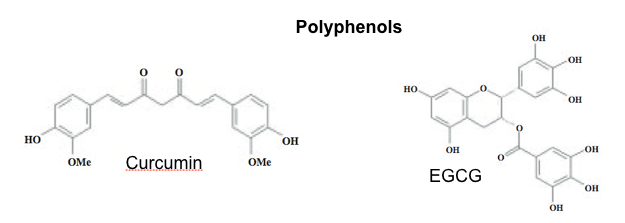
\includegraphics[width=6in]{figures/introduction/polyphenols.png}
\caption[Small molecule binders]{Polyphenols}
\label{fig:polyphenols}
\end{figure}

\subsection{Polyphenols}
Polyphenols,  is a large group of natural and synthetic molecules.  (−)-epigallocatechin-3-gallate, curcumin, and a polyphenolic grape seed extract, known for their anti-oxidant properties,  were recently discovered to be capable of affecting amyloid formation.(Fig.~\ref{fig:polyphenols})

\subsection{Inositol}
\begin{figure}
\centering
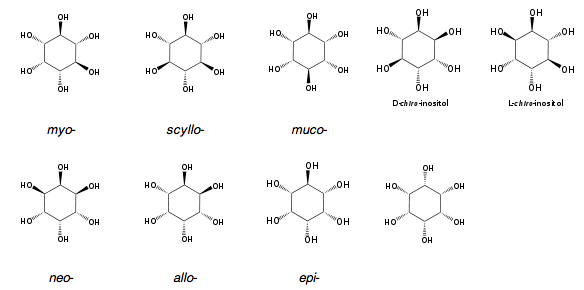
\includegraphics[width=6in]{figures/introduction/inositol.png}
\caption[Inositol]{Inositol stereoisomers}
\label{fig:inositols}
\end{figure}

% Should tell a little story of how inositol was discovered.  I remember that Chris Yip thought this might have been nice ... because it seems out of the blue to people.

% What I wrote in my transfer proposal:

Inositol with the molecular formula of \ce{C_6H_12O_6}, is a simple polyol with nine naturally occurring stereoisomers. Out of these nine isomers, seven are optically inactive, and the remaining two (L- and D-chiro-inositol) are chiral enantiomers.(Figure~\ref{fig:inositols})

% Here, use the physiological role of myo-inositol as a lead to transition into its role in amyloid inhibition.

Myo-inositol, the most abundant isomer, is ubiquitous in all eukaryotes and is a physiologically important osmolyte.  Furthermore, myo- is a precursor for inositol lipid synthesis: It is a constituent of phosphatidylinositol, an important phospholipid in membranes and second messenger systems. Once phosphorylated, myo-inositol phosphatides act as second messengers in intracellular signal transduction pathways.\cite{Fisher:2002tk}

Inositol is found in high concentrations in tissues of the human central nervous system (CNS): myo- And scyllo-inositol have approximate concentrations of 5 and 0.1-0.5 mM in the CNS, respectively.\cite{Fisher:2002tk} Accordingly, inositols also function as osmolytes in the CNS, where alterations in their concentrations are known to be associated with neuropathological conditions.\cite{Michaelis:1993gf, Fisher:2002tk}

% Role of inositol in amyloid inhibition. Here, include the background on how inositol was discovered as an \abeta\ amyloid fibril inhibitor
In recent years, scyllo-inositol have been identified as a promising therapeutic candidate for the treatment of Alzheimer's Disease.

Scyllo-, myo-, and epi-, but not chiro-inositol, have been shown to inhibit \abeta42 fibril assembly, stabilize an oligomeric complex of \abeta42, and attenuate \abeta-oligomer-induced neurotoxicity in vitro. Moreover, inositol exhibits stereochemistry-specific effects on \abeta\  fibril inhibition and cytotoxicity: scyllo- and epi- are more effective than myo-inositol, whereas chiro-inositol was inactive.\cite{McLaurin:2000bq}

An important therapeutic advantage of scyllo-inositol is its ability to readily crosses the bloodbrain barrier (BBB) (both actively and passively transported). Because it is not enzymatically broken down in the gut, it may be administered as a drug orally. 
% Inositol is synthesized inside the body ... or can be obtained via nutrition?  
		
In vivo studies with a transgenic mouse model of AD demonstrated that alleviation of symptoms after inositol treatment was correlated with a decrease in the levels of soluble \abeta\ oligomers, suggesting that the beneficial effects of scyllo-inositol may be attributed to the inhibition and/or disaggregation of high-order \abeta\ oligomers.\cite{McLaurin:2006eb}

Taken together, these results suggest that scyllo-inositol, and its derivatives, are a potential therapy for AD with the ability to change the course of the disease.\cite{Nitz:2008jl,Sun:2008ko}

% Include some data on human clinical trials (?) -- II was negative ... how to say it ? Should read phase II paper.
Presently scyllo-inositol completed both phase I and II of human clinical trials, where it was demonstrated that inositol is not toxic to healthy individuals at concentrations effective for amyloid inhibition.

\subsection{Commonalities between small molecule inhibitors}
% Commonalities between small molecules which appear to affect amyloid aggregation
Small molecule inhibitors share common chemical features and groups.  They are typically planar in geometry, have many aromatic rings, and polar functional groups (hydroxyl groups) around the edge of these aromatic rings.



\subsection{Molecular mechanisms of amyloid inhibition 
	            \\ by small molecules}
% Mechanism of action.
Some small molecules inhibit fibril formation, where as others may prevent oligomerization, but not fibrillation. A high concentration is often required to observe activity (micromolar to millimolar), which suggests that they may be non-specific inhibitors. EGCG, one such polyphenol, is known to have the lowest IC50.
    	% IC50 -- This quantitative measure indicates how much of a particular drug or other substance (inhibitor) is needed to inhibit a given biological process (or component of a process, i.e. an enzyme, cell, cell receptor or microorganism) by half.
      % EC50 -- The term half maximal effective concentration (EC50) refers to the concentration of a drug, antibody or toxicant which induces a response halfway between the baseline and maximum after some specified exposure time.[1] It is commonly used as a measure of drug's potency.
      % Ref: wikipedia
      
  	% Review of what is known about amyloid fibril ligand binding, specifically dyes.

Molecular mechanism of binding of dye molecules. Thought to bind flat on on the surface grooves of amyloid fibrils where they interact with hydrophobic groups exposed at the surface. 
      % Doesn't explain why the dye molecules are also able to suppress fibril formation.
      % Can the birefringence be explained by these binding modes? -- this is out of the scope of my thesis.  Don't put this in my thesis but I should be able to coherently explain this during my defense.

\section{Analogy to Sugar-protein binding}
% Does this section fit here? Where should I put it?
% Could use this as a prime example of protein-ligand interaction ...
% As a prime example of protein ligand interaction, one of the first systems that was used to understand binding was a sugar binding protein lysozyme ... -- No I think I will use early systems used to understand protein-ligand binding and if that was a sugar binding protein, then it will come off as a coincidence.
% This section is best discussed in the context of understanding inositol binding ...

% Mention some experimental techniques used to obtain protein sugar-binding modes, but the point here is not to review these methods ... but to point out that I am aware of these techniques.

\subsection{Sugar Binding modes}

% This section provides a nice lead in to the methods section
\section{Protein-ligand interactions}
\subsection{Forces involved in binding}
% Note that I may end up introducing the forces up in the earlier section -- reorganize as needed
\begin{outline}
	\1 Protein-ligand non-covalent interactions that are important for ligand binding and recognition
		\2 Electrostatic interactions. Polar (hydrogen bonding) and charge-charge interactions
		 % Here, it will benefit me to read Sarah's appendix C carefully.
		\2 Nonpolar (hydrophobic) interactions
		  \3 Van der Waals
\end{outline}

\subsection{Binding equilibria}
% subsection protein_ligand_binding_theory (end)
% Below is a summary of an excerpt from Tom's thesis on structure-based drug discovery.
% Design of antibiotics 
% 1) Target determination (biochemical)
% 2) Structural determination (Xray, NMR, or homology); active site identified; Here would be useful to get the holo structure of the protein
% 3) Screen for inhibitors against a chemical library or in silico docking.
\begin{outline}
	\1 Enzyme and its putative ligand typically bind specifically (high affinity binding).  We want to optimize binding specificity to increase the efficacy of the putative drug, and decrease adverse side effects (toxicity) in the human body.

	\1 The dissociation constant, $K_d$, is a measure of the affinity of a ligand for its binding site on the host protein. Pharmacologically, it can be interpreted as the concentration at which 50\% of the drug is bound to the protein. In experimental studies, $K_d$ is often used to quantitatively screen for potential drug candidates. 
  % A small $K_d$ suggests that the ligand may bind tightly to the protein.

	\1 Binding equilibrium

    \begin{equation}
      \left[ Protein\cdot Inositol \right] 
      \rightleftharpoons 
      \left[ Protein \right]+\left[ Inositol \right]
    \end{equation}
  
    % \2 Absolute binding free energy
    % \2 Relative binding free energy
    
	\1 The binding free energy of a ligand to a protein is directly related to its dissociation constant, $K_d$, the equilibrium constant of the above reaction

     \begin{equation}
        K_{d} = f_{ub}\frac{\left[ Protein \right]\left[ Inositol \right]}{\left[Protein \cdot Inositol\right]},
     \end{equation}
     
     % Add equation converting binding constant to gibbs free energies.
	\1 Experimental techniques for estimating $K_d$
		\2 What experimental techniques are used to estimate binding affinity? (May need to study up on this)
		\2 Isothermal titration calorimetry (ITC) is a technique which can be used to measure energetics of ligand binding to peptides.
\end{outline}

% \subsection{Role of chirality in drug binding}
% Stereoisomerism is important to the activity of molecules.  It modulates binding to proteins.
% Two types of stereochemistry
% Constitutional isomers - differs in bonding sequences and connectivity
% Stereoisomers - differs in orientation of their atoms in space, but no connectivity differences.
% Definition of chirality [Add schematic] ... etc
% Molecules with chirality have a non-superimposable mirror image, called an enantiomer.
% A carbon molecule with four different groups has chirality.

\section{Thesis objectives and rationale}
% Understanding amyloid inhibition in the context of the framework of traditional enzyme inhibition mechanism
\subsection{Challenges of amyloid inhibition}
\begin{outline}
       % However, most of these studies were focused on A$\beta$ and large A$\beta$ aggregates,\{Fawzi, 2008 \#553;Esposito, 2008 \#567;Sgourakis, 2007 \#609;Wei, 2006 \#656;Tarus, 2006 \#628 Karsai, 2006 \#658\} and thus, were computationally limited by the complexity of the molecular systems.

    \1 The protein-ligand binding model developed to understand enzyme inhibition cannot be directly applied to understand the molecular mechanism of amyloid inhibition by small molecules. 
    
      \2 Amyloid inhibitors are found to be very weak binders. How do non-specific inhibitors act as a drug? And how do we approach this with MD simulations?
      
      \2  Because the A$\beta$ amyloid aggregate pathway encompasses a variety of species, some of which has no folded structure, a single conformation cannot be assumed for binding. Furthermore, structural information of amyloidogenic species lags behind those of enzymes, which tends to be globular proteins amenable for X-ray crystallography. This means that the putative binding sites are not known.
      
      \2 The structural disorder of the peptides involved poses a challenge for obtaining converged properties from MD simulations. 
    
    	\1 A$\beta$ peptides are completely disordered.  We also do not know what the binding site looks like, where it is located on these structures.
    	
    \1 To date, few studies have attempted to provide statistically meaningful results pertaining to general mechanisms of protein self-aggregation and amyloid formation. Furthermore, despite the abundance of MD studies of A$\beta$, few studies have systematically examined the mechanism of action of small molecule inhibitors of amyloids

    \1 In AD, there is the added challenge of the drug being able to cross the brain barrier, while remaining non-neurotoxic.  What kind of drugs cross the BBB?  Typically hydrophobic drugs.
\end{outline}    

\subsection{Study Design and Rationale}
\begin{outline}
	\1 Here describe in detail how I designed my study to circumvent the challenges presented by the amyloid inhibition problem, and the limitations  of MD simulations. At this point, clearly explain and discuss my study design and rationale. (Fig.~\ref{fig:rationale})

  \begin{figure}
    \centering
    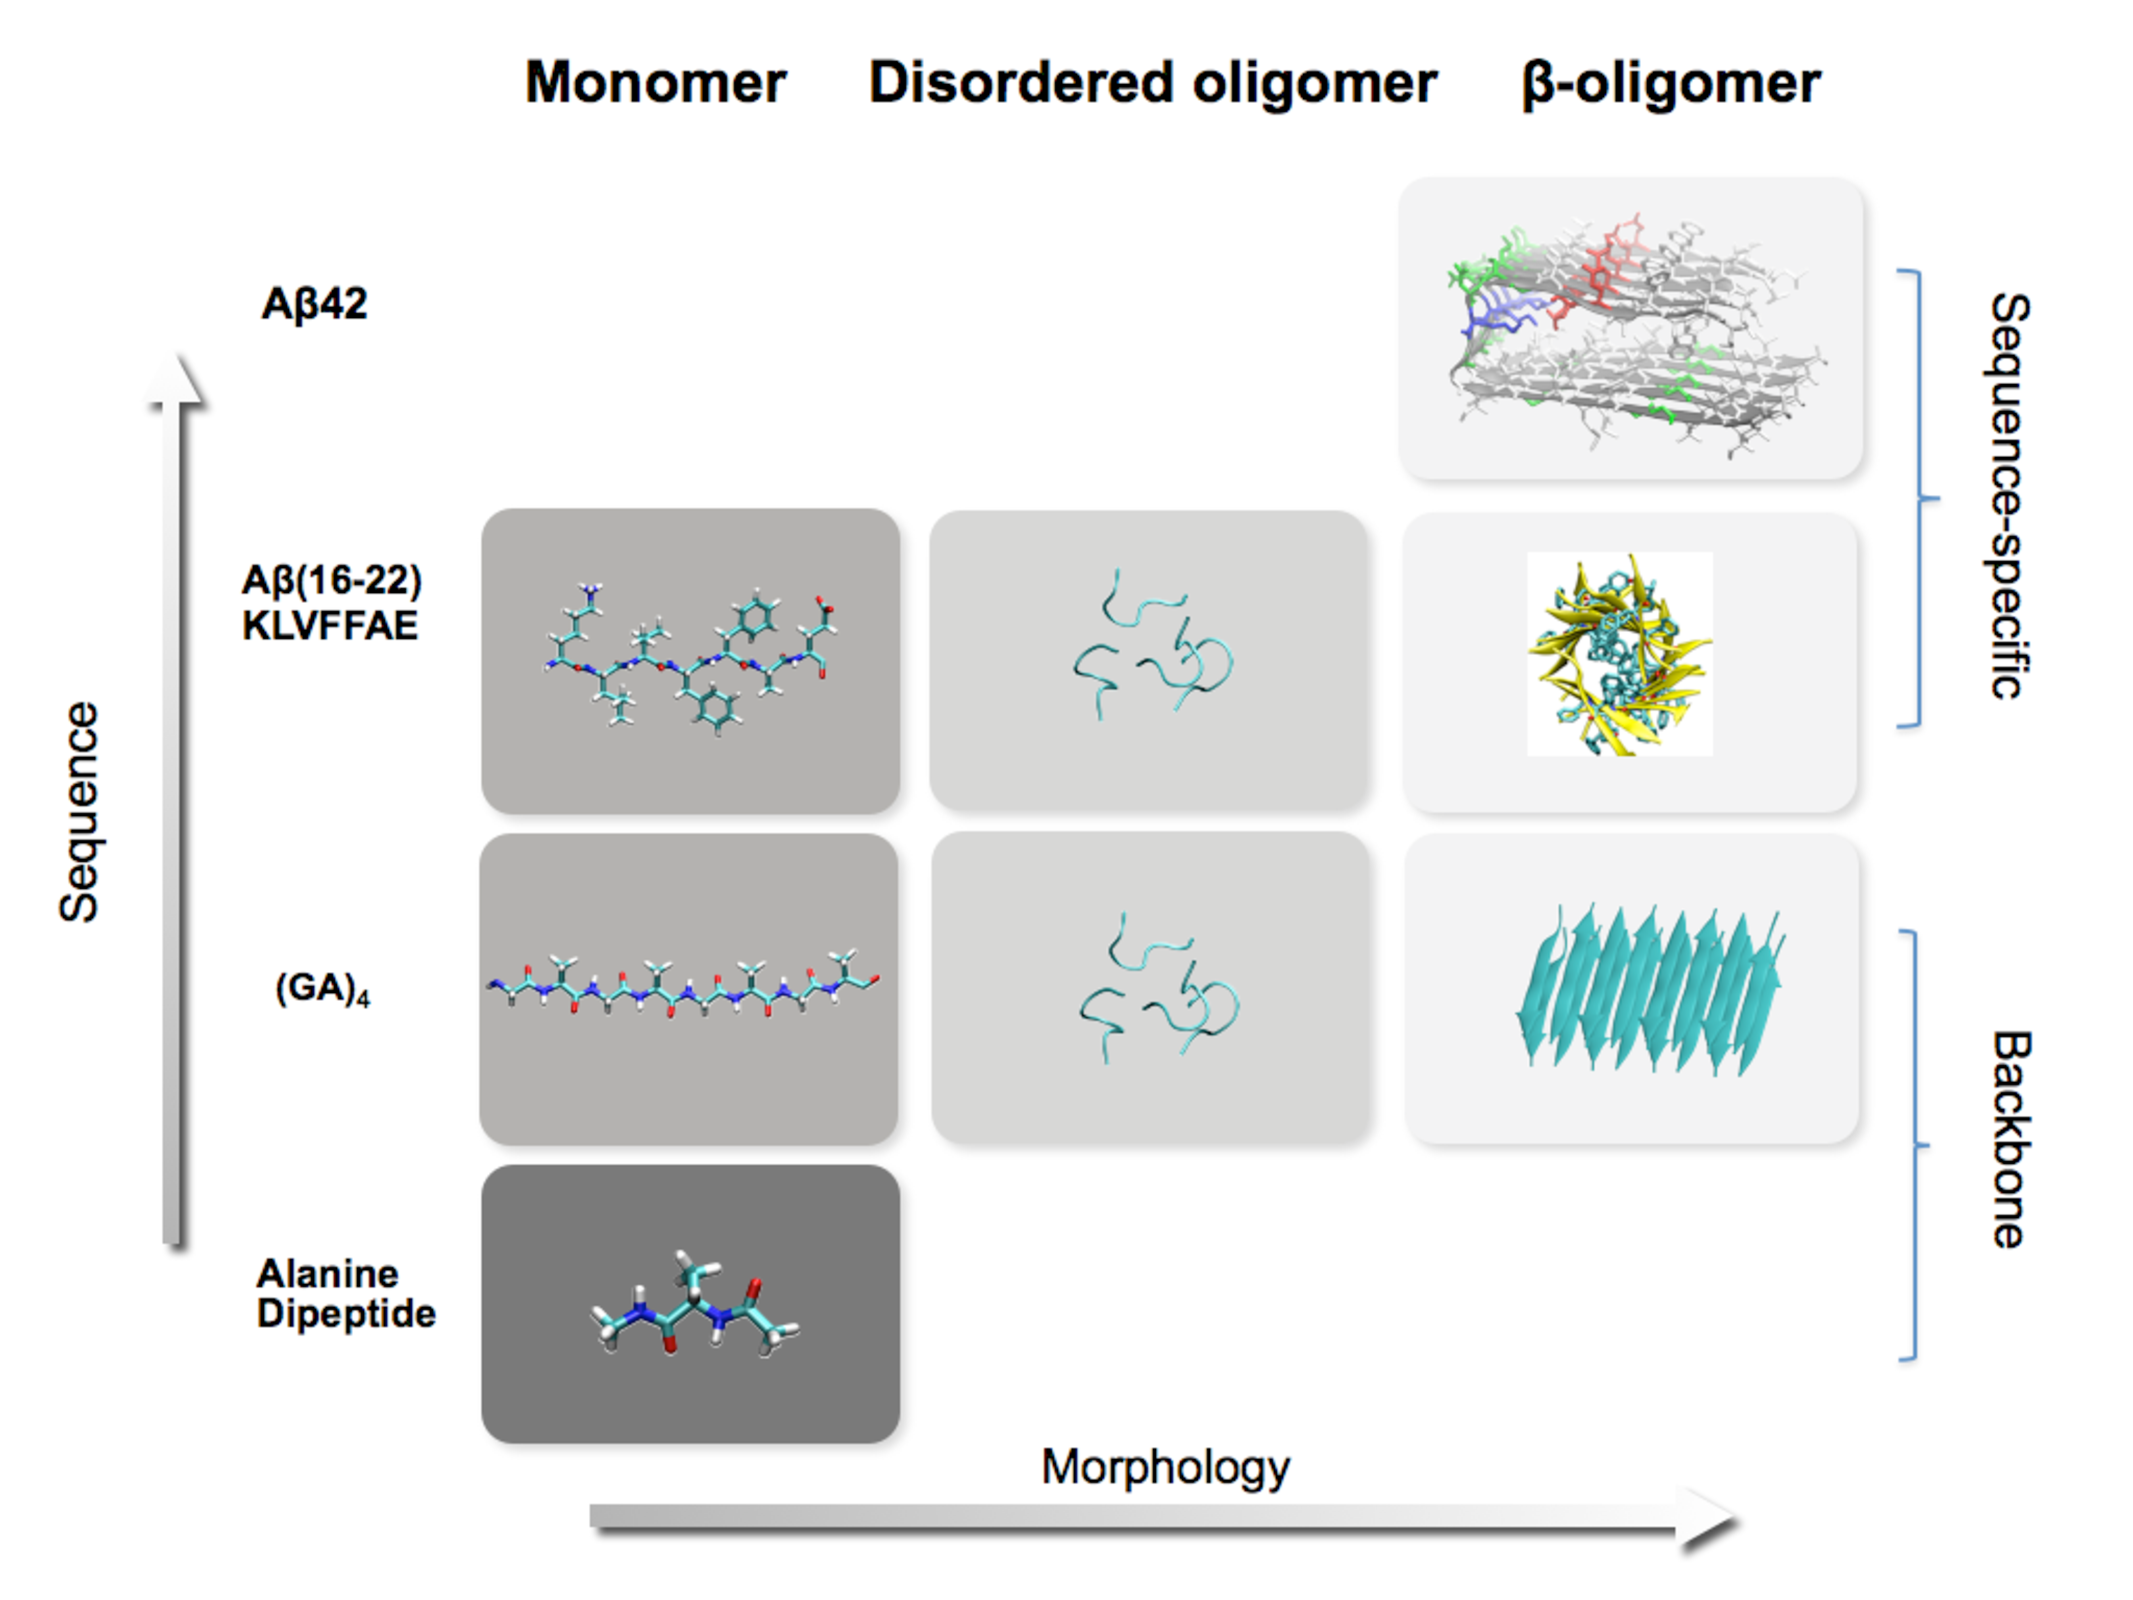
\includegraphics[width=6in]{figures/introduction/matrix.pdf}
    \caption[Rationale]{Shows the progression from small, model systems to larger and structurally more complex systems involving the full-length A$\beta$42 peptide.}
    \label{fig:rationale}
  \end{figure}

	\1 Beginning with the simplest model systems for an amyloidogenic peptide, the alanine dipeptide, we systematically examine binding of inositol with systems of both increasing sequence and structural complexity.

	% Use brute force simulations
	\1 We exploit conventional MD simulation techniques because simulation approaches used for understanding enzyme-ligand binding is not applicable. 
	
	\1 Instead, we use conventional MD simulations and repeats of independent simulations to determine the binding modes, and binding equilibria of inositol with amyloidogenic peptides and aggregates of A$\beta$.
\end{outline}

\section{Thesis Organization}
The first chapter introduces the thesis in the context of the field.  The second chapter introduces the main methods used in the work in the thesis. Chapters 3, 4, and 5 are the results of simulations of inositol with amyloid like peptides and aggregates. Chapter 6 shows work of the general applicability of our methods developed throughout this thesis to MD simulations to understand protein - carbohydrate binding. Chapter 7 provides discussion, suggestions for future work, and perspectives.

\addcontentsline{toc}{section}{Bibliography}
\bibliographystyle{plain}
\bibliography{chapter1}

% AD
% Treatment - harder to treat - lack of biochemical understanding of what causes disease, which makes it difficult to develop drugs for; lack of good diagnostic methods because treatment may not be effective at end stages of the disease where brain function won't e able to be rescued.
% Diagnosis - hard to diagnose
% AD is difficult to diagnose.  It is often not apparent that someone has AD until they exhibit symptoms severe enough to interfere with daily life or occupation. 

% Amyloid hypothesis - our best guess at what causes AD and provides the best guess at what we should be targeting. 
% Abeta Amyloid thus far provides the best clue to the molecular basis of AD, and thus a promising pathway to a cure for AD.

% In some individuals without dementia symptoms may have as much plaque as another with severe AD. Synaptic loss can be used as a measure of disease progression. 

% Perhaps use this as a transition into the general discussion of amyloid formation and structure -- not only specific to Abeta.
% Furthermore, amyloid have also been known to play beneficial roles in certain living systems. REF
% Increasing awareness of the amyloid state of proteins, and interest grew in amyloids because of their role in a variety of devastating human diseases.

% Fibrils

% In this section I will talk about how amyloid aggregation is thought to work. Introduce the thermodynamic model for understanding fibril formation.